\chapter{Реализация и экспериментальная проверка работоспособности модуля}

\section{Реализация анализатора плагинов Terraform}

Для реализации анализатора плагинов Terraform был использован язык
программирования Go, так как Terraform и большинство его плагинов написаны на
Go.

Анализатор плагинов Terraform реализован как отдельное приложение на Go, которое
анализирует исходный код плагинов Terraform и извлекает из него метаданные,
необходимые для генерации классов-оберток на Scala.

В основе анализатора лежит рефлексия - механизм, позволяющий программам
исследовать структуру кода во время выполнения. С помощью рефлексии анализатор
исследует структуру плагина Terraform, извлекает информацию о типах ресурсов и
их свойствах и преобразует эту информацию в формат, подходящий для генерации
классов-оберток на Scala.

В процессе анализа анализатор обходит все структуры и поля в плагине,
обрабатывая каждое поле в зависимости от его типа. Для структур и отображений
(map) анализатор рекурсивно обходит их поля, для срезов (slice) - их элементы.
Функции и другие необрабатываемые типы пропускаются.

Результат работы анализатора - файл JSON с метаданными плагина, который затем
используется модулем генерации классов-оберток для создания классов-оберток на
Scala.

Код анализатора находится в Приложении \ref{sec:appendix1}.

В этом коде функции обхода структур (walkStruct), обхода срезов (walkSlice) и
обхода отображений (walkMap) используются для обхода соответствующих структур
данных. Они вызывают функцию обработки значения (processValue) для каждого поля
или элемента, которая в свою очередь обрабатывает значение в зависимости от его
типа и возвращает его в формате, подходящем для записи в JSON.

Функция проверки допустимости значения (valueIsValid) используется для
определения, является ли значение обрабатываемым. Она возвращает false для
функций и других типов значений, которые не могут быть корректно преобразованы в
JSON.

В главной функции (main) происходит инициализация плагина Terraform, извлечение
информации о провайдере с помощью рефлексии, преобразование этой информации в
JSON и запись JSON в файл.

Пример файла JSON с метаданными плагина Terraform см. в Приложении
\ref{sec:appendix2}.

Таким образом, анализатор плагинов Terraform позволяет извлечь из плагинов
метаданные, необходимые для генерации классов-оберток на Scala. Эти метаданные
включают в себя информацию о типах ресурсов и их свойствах, которые затем
используются при генерации кода на Scala.

\section{Реализация анализатора документации}

Анализатор документации реализован на языке Python и использует библиотеки json,
os, re и hcl. Он проходит через все файлы в указанной директории, извлекает
блоки кода конфигурации Terraform (HCL) из файлов с расширением .md или
.markdown, анализирует их и сохраняет результат в формате JSON.

Вот основные шаги работы анализатора:

\begin{itemize}
  \item Извлечение блоков кода конфигурации Terraform из файлов документации.
Это достигается с помощью функции извлечения блоков кода из директории
(extract\_code\_blocks\_from\_directory), которая проходит через все файлы в
указанной директории и вызывает функцию извлечения блоков кода из файла
(extract\_code\_blocks\_from\_file) для каждого файла. Функция извлечения блоков
кода из файла открывает файл, читает его содержимое и использует регулярное
выражение для поиска блоков кода конфигурации Terraform.
  
  \item Анализ блоков кода конфигурации Terraform. Это делается с помощью
функции анализа конфигурации Terraform (parse\_terraform), которая принимает на
вход массив блоков кода конфигурации Terraform и пытается проанализировать
каждый из них с помощью библиотеки hcl. Если анализ проходит успешно, результат
добавляется в массив проанализированных блоков (hcl\_arr).
  
  \item Преобразование сложных структур данных в плоский формат. Это делается с
помощью функции выравнивания словаря (flatten\_dict), которая принимает на вход
словарь и преобразует его в плоский формат, где каждый ключ представляет собой
путь к соответствующему значению в исходном словаре.
  
  \item Сохранение результатов в файл. После обработки всех блоков кода
конфигурации Terraform результаты сохраняются в файл в формате JSON.
\end{itemize}

Полный код анализатора представлен в Приложении \ref{sec:appendix3}.

Пример файла JSON с метаданными документации Terraform см. в Приложении
\ref{sec:appendix4}.

\section{Реализация модуля генерации классов-оберток}

Модуль состоит из многих файлов, опишем основные из них в текущем разделе.

\subsection{Реализация анализатора документации}

Модуль анализатора документации отвечает за обработку и анализ документации в
формате JSON, полученной из Terraform. Он использует библиотеку Circe для
декодирования JSON и библиотеку Scala для работы с регулярными выражениями и
файлами.

Вот основные компоненты этого модуля:

\begin{itemize}
  \item JsonValue: это абстрактный класс, представляющий значение JSON. Он имеет
четыре подкласса: JsonString, JsonBool, JsonLong и JsonDouble, которые
представляют соответствующие типы данных JSON.

  \item JsonMap: это тип для представления отображения JSON, где ключи - это
строки, а значения - это списки значений JSON.
  
  \item DocsInfo: это класс, который содержит информацию, извлеченную из
документации. Он содержит различные отображения для хранения доменов,
IP-адресов, масок IP-адресов, строк JSON и ссылок на поля.
  
  \item decodeJsonMap: эта функция декодирует строку JSON в JsonMap. Если
происходит ошибка декодирования, она выбрасывает исключение.
  
  \item filterJsonMap: эта функция фильтрует JsonMap, оставляя только ключи,
которые начинаются с "output.", "resource." или "data.".
  
  \item definePatterns: эта функция определяет регулярные выражения для
различных типов значений, таких как поля, домены, IP-адреса и маски IP-адресов.
  
  \item decodeAndFilterJson: это основная функция модуля. Она принимает строку
JSON, декодирует ее в JsonMap, фильтрует отображение, извлекает различные типы
значений и возвращает DocsInfo с этой информацией.
\end{itemize}

\subsection{Описание классов и функций}

Основные классы представлены на рисунке \ref{fig:uml1}.

\begin{figure}[h]
  \centering
  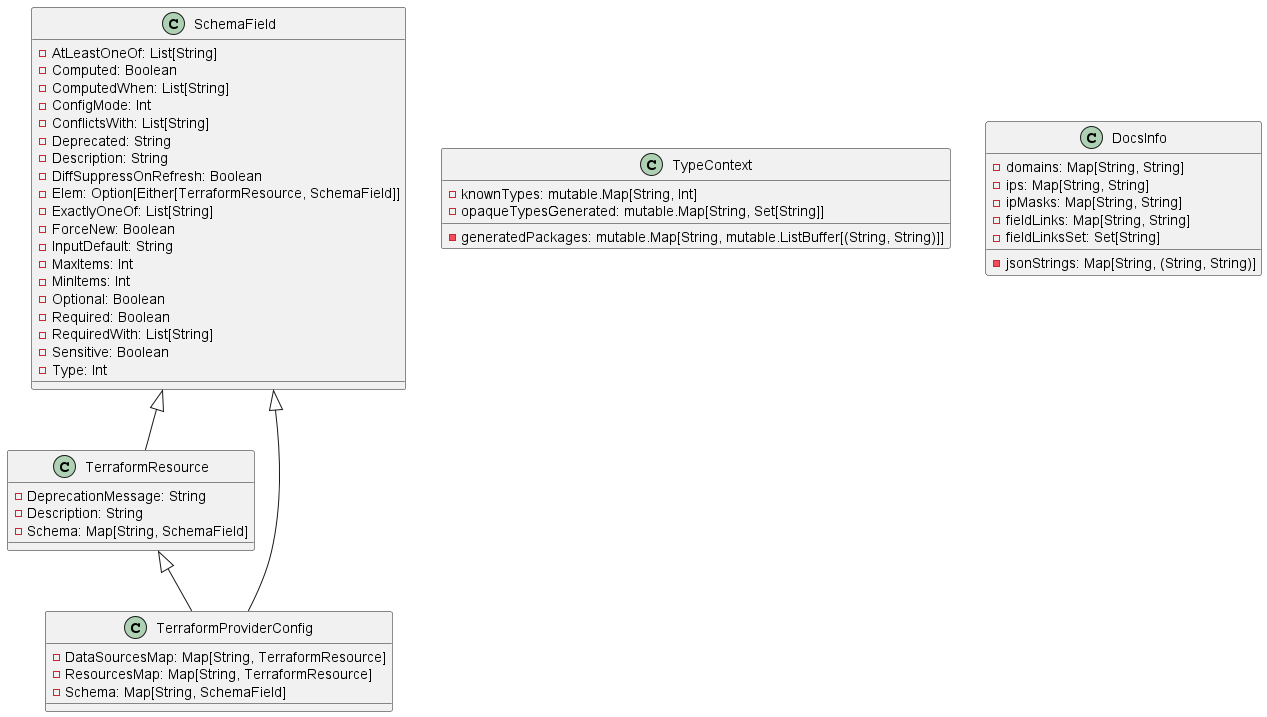
\includegraphics[scale=0.35]{img/5.png}
  \caption{Основные классы модуля генерации классов-оберток}
  \label{fig:uml1}
\end{figure}

\vspace{60mm}

Далее опишем основные классы и функции модуля:

\begin{itemize}
  \item SchemaField: Этот класс представляет собой модель для полей схемы в
Terraform. Он содержит различные атрибуты, такие как AtLeastOneOf, Computed,
ComputedWhen, ConfigMode, ConflictsWith, Deprecated, Description,
DiffSuppressOnRefresh, Elem, ExactlyOneOf, ForceNew, InputDefault, MaxItems,
MinItems, Optional, Required, RequiredWith, Sensitive, Type. Elem - это
опциональное поле, которое может содержать либо TerraformResource, либо другой
SchemaField.
  
  \item TerraformProviderConfig: Этот класс представляет конфигурацию провайдера
Terraform. Он содержит отображения для DataSourcesMap, ResourcesMap и Schema.
  
  \item TerraformResource: Этот класс представляет ресурс в Terraform. Он
содержит DeprecationMessage, Description и Schema.
  
  \item TypeContext: Этот класс содержит контекст для типов, включая knownTypes,
generatedPackages и opaqueTypesGenerated.
  
  \item DocsInfo: Этот класс содержит информацию, извлеченную из документации
Terraform. Он содержит отображения для domains, ips, ipMasks, jsonStrings,
fieldLinks и множество fieldLinksSet.
  
  \item TypeCodes: Этот объект содержит константы для различных типов полей.
  
  \item generateFieldType: Эта функция генерирует тип поля на основе
SchemaField.
  
  \item updateFieldWithType: Эта функция обновляет поле с типом на основе
SchemaField.
  
  \item generateTodoComment: Эта функция генерирует комментарий TODO для поля.
  
  \item generateSchemaForElem: Эта функция генерирует схему для элемента на
основе SchemaField.
  
  \item generateSchemaField: Эта функция генерирует поле схемы на основе
SchemaField.
  
  \item generateResourceClassName: Эта функция генерирует имя класса ресурса.
  
  \item generatePackageName: Эта функция генерирует имя пакета.
  
  \item generateFullName: Эта функция генерирует полное имя.
  
  \item generateFields: Эта функция генерирует поля для ресурса.
  
  \item getUniqueClassName: Эта функция генерирует уникальное имя класса.
  
  \item generateToHCLBody: Эта функция генерирует тело метода toHCL.
  
  \item generateToHCLMethod: Эта функция генерирует метод toHCL.
  
  \item generateFieldDescriptions: Эта функция генерирует описания полей для
ScalaDoc.
  
  \item generateClassDoc: Эта функция генерирует документацию для класса,
включая описание ресурса и описания полей.
  
  \item generateDeprecationAnnotation: Эта функция генерирует аннотацию
устаревания, если ресурс устарел.
  
  \item generateClassDef: Эта функция генерирует определение класса, включая его
поля и методы.
  
  \item generatePackageCode: Эта функция генерирует код пакета, включая
определения классов и связанных полей.
  
  \item updateContext: Эта функция обновляет контекст, добавляя новые классы и
пакеты.
  
  \item generateLinkedFields: Эта функция генерирует связанные поля для ресурса.
  
  \item generateResourceClass: Эта функция генерирует класс ресурса на основе
конфигурации ресурса.
  
  \item generateCaseClasses: Эта функция генерирует классы-обертки для
конфигурации провайдера.
  
  \item generateDataSources: Эта функция генерирует источники данных для
конфигурации провайдера.
  
  \item generateResources: Эта функция генерирует ресурсы для конфигурации
провайдера.
  
  \item generateProviderResource: Эта функция генерирует ресурс провайдера для
конфигурации провайдера.
  
  \item printFieldLinksInfo: Эта функция выводит информацию о связанных полях.
  
  \item generatePackages: Эта функция генерирует пакеты на основе контекста.
  
  \item generateProviderPackage: Эта функция генерирует пакет провайдера.
\end{itemize}

Код для данного модуля не будет приведен в текущей статье из-за его большого
объема. Полный код доступен в репозитории проекта.

\subsection{Пример работы}

В этом примере мы используем библиотеку Circe для декодирования JSON,
представляющего конфигурацию провайдера Terraform, и генерируем соответствующие
классы Scala.

Сначала мы читаем JSON из файла и декодируем его в объект
TerraformProviderConfig. Затем мы генерируем классы Scala для каждого ресурса и
источника данных в конфигурации провайдера с использованием функции
generateCaseClasses. Наконец, мы записываем сгенерированный код Scala в файлы в
соответствующих пакетах.

Пример кода см. в Приложении \ref{sec:appendix6}.

Диаграмма классов для сгенерированного кода Scala представлена на рисунке
\ref{fig:uml2}.

\begin{figure}[h]
  \centering
  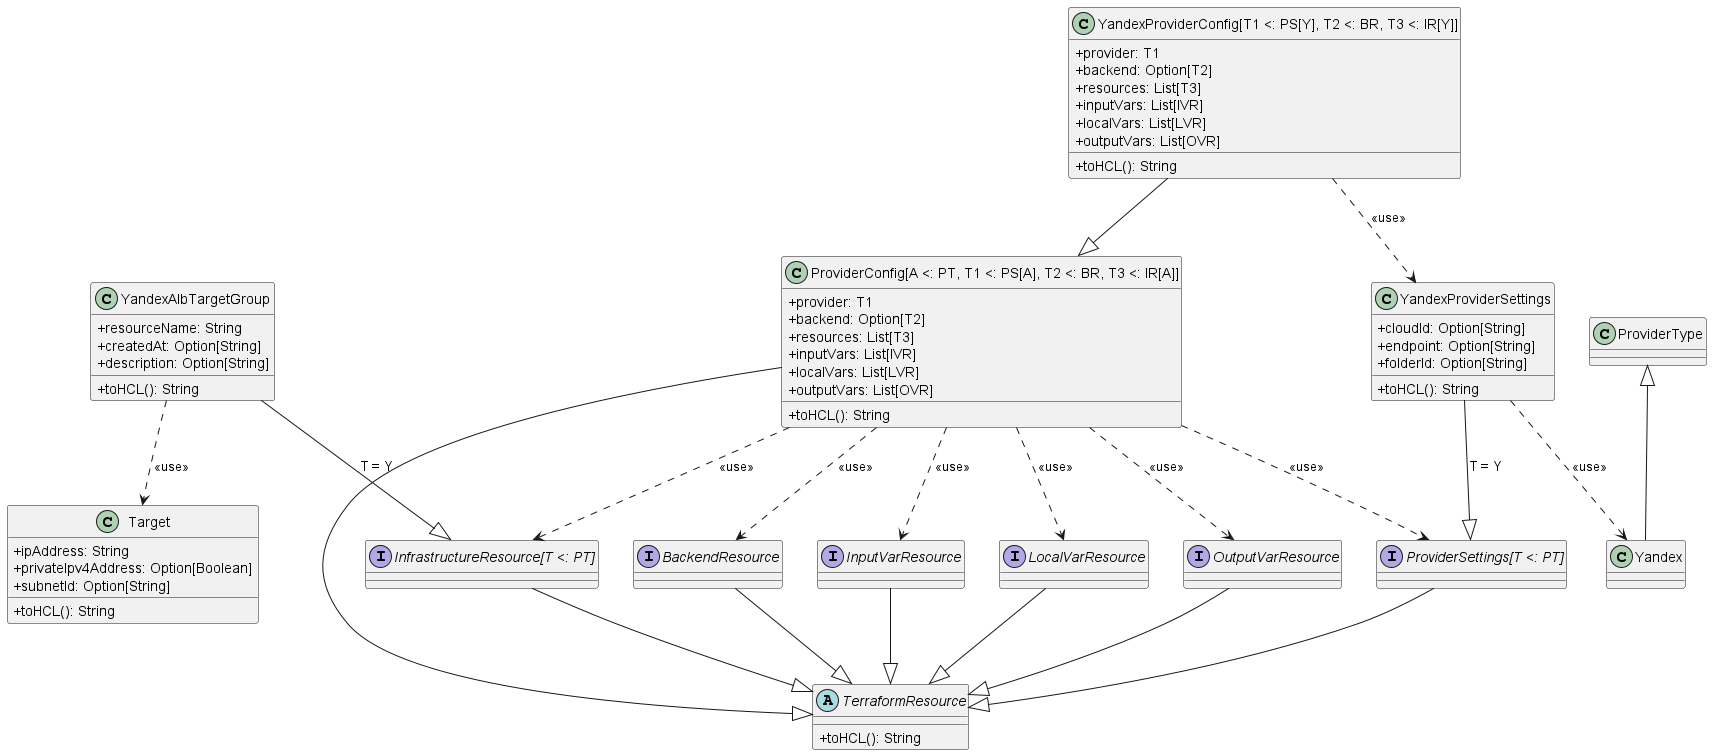
\includegraphics[scale=0.25]{img/6.png}
  \caption{Диаграмма классов для сгенерированного кода Scala}
  \label{fig:uml2}
\end{figure}

В этом примере мы используем файлы JSON, сгенерированные с помощью инструментов
извлечения документации Terraform и преобразования конфигурации Terraform в
JSON, для представления конфигурации провайдера Terraform и связанных с ним
документов. Эти файлы затем используются для генерации классов Scala, которые
могут быть использованы для работы с этим провайдером в Scala.

\section{Реализация модуля для работы с программным интерфейсом Kubernetes}

\subsection{Описание классов}

В данном модуле определены следующие классы:
\begin{itemize}
  \item AllocatedResources: Этот класс представляет выделенные ресурсы. Он
содержит следующие поля: cpuRequests (запросы процессорного времени), cpuLimits
(ограничения процессорного времени), memoryRequests (запросы памяти),
memoryLimits (ограничения памяти), ephemeralStorageRequests (запросы эфемерного
хранилища), ephemeralStorageLimits (ограничения эфемерного хранилища),
hugepages2MiRequests (запросы огромных страниц размером 2 Ми),
hugepages2MiLimits (ограничения огромных страниц размером 2 Ми),
hugepages1GiRequests (запросы огромных страниц размером 1 Ги),
hugepages1GiLimits (ограничения огромных страниц размером 1 Ги). Все поля имеют
тип BigDecimal.
  
  \item ContainerStates: Этот класс представляет состояния контейнера. Он
содержит одно поле: id (идентификатор) типа String.
  
  \item PodConditions: Этот класс представляет условия модуля (пода). Он
содержит следующие поля: conditionType (тип условия) типа String и status
(статус) типа Boolean.
  
  \item MyPod: Этот класс представляет модуль (под). Он содержит следующие поля:
ip (IP-адрес) типа Option[String], name (имя) типа String, status (статус) типа
Option[String], startedAt (время запуска) типа Option[String], createdAt (время
создания) типа Option[String], age (возраст) типа Option[String], ageInSec
(возраст в секундах) типа Long, restarts (перезапуски) типа Int, states
(состояния) типа List[ContainerStates], allocatedResources (выделенные ресурсы)
типа AllocatedResources, namespace (пространство имен) типа String, isSystem
(системный) типа Boolean, failedScheduling (не удалось запланировать) типа
Boolean, events (события) типа Map[String, MyEvent], conditions (условия) типа
List[PodConditions], uid (уникальный идентификатор) типа String.
  
  \item MyNode: Этот класс представляет узел. Он содержит следующие поля: name
(имя) типа String, status (статус) типа Map[String, Boolean], pods (модули) типа
Map[String, MyPod], ip (IP-адреса) типа Map[String, String], allocatedResources
(выделенные ресурсы) типа AllocatedResources, capacity (емкость) типа
Map[String, BigDecimal], allocatable (доступно для выделения) типа Map[String,
BigDecimal], uid (уникальный идентификатор) типа String.
  
  \item KuberInfo: Этот класс представляет информацию о кластере Kubernetes. Он
содержит следующие поля: nodes (узлы) типа Map[String, MyNode], podsWithoutNode
(модули без узла) типа Map[String, MyPod], unscheduledPods (незапланированные
модули) типа Map[String, MyPod], events (события) типа List[MyEvent], namespaces
(пространства имен) типа Set[String].
  \end{itemize}
  
  UML-диаграмма для классов представлена на рисунке \ref{fig:uml3}.
  
  \begin{figure}[h]
   \centering
   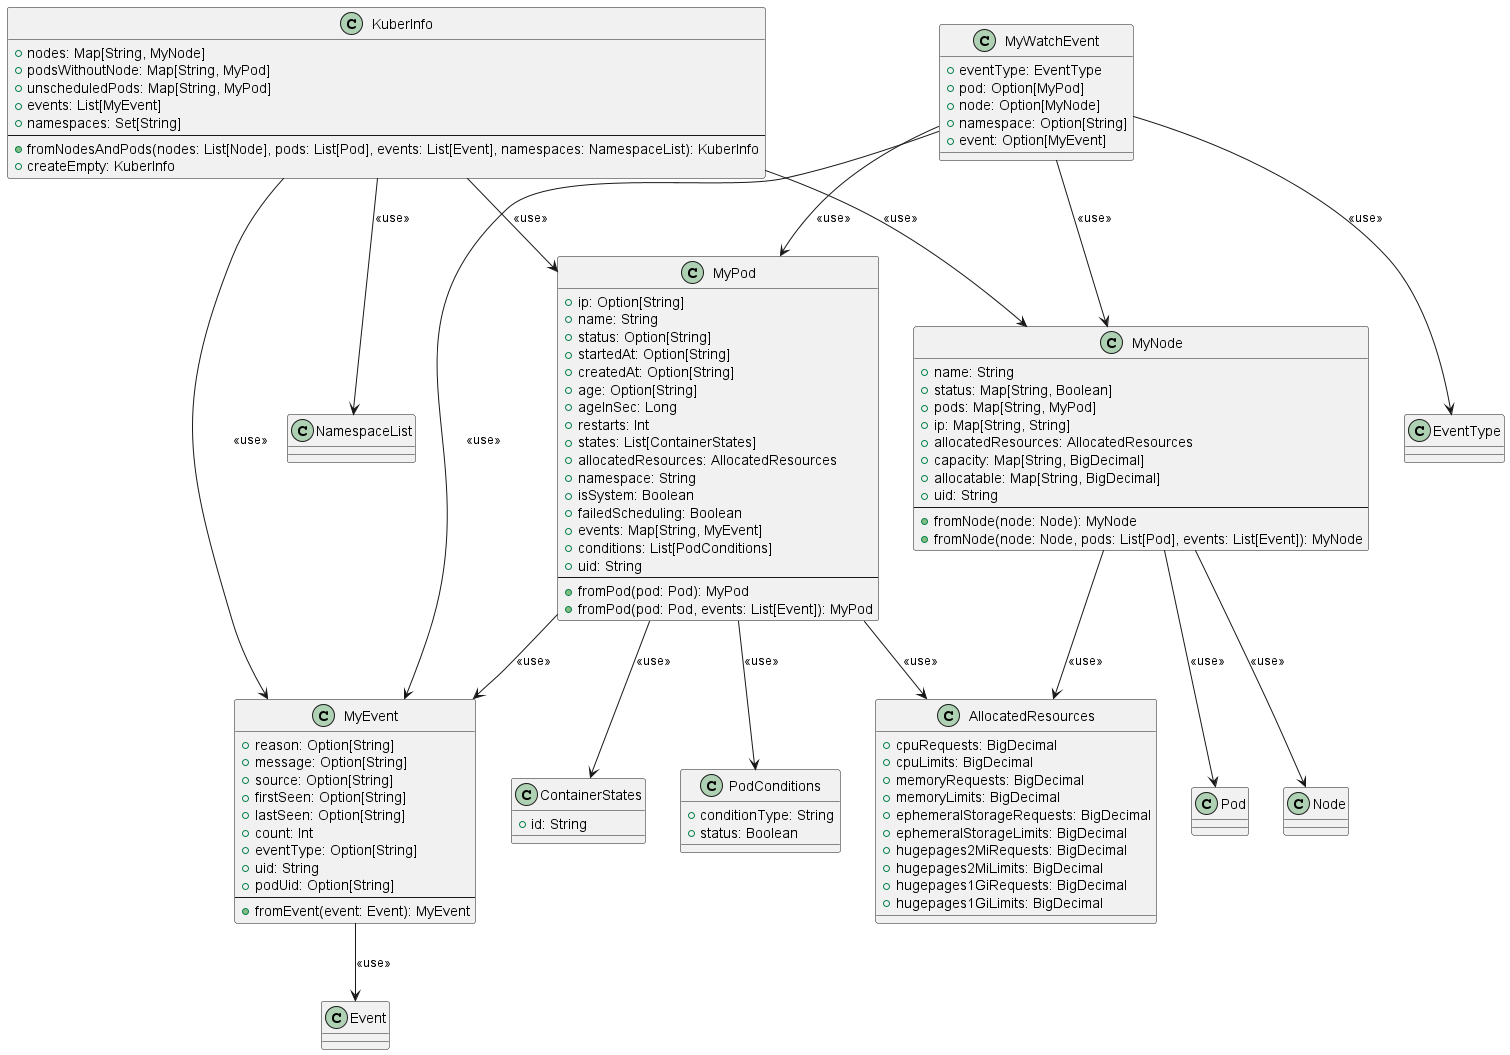
\includegraphics[scale=0.3]{img/7.png}
   \caption{Диаграмма классов модуля автомасштабирования}
   \label{fig:uml3}
  \end{figure}
  
  \subsection{Описание методов}
  
  \begin{itemize}
  \item waitUntilAllPodsVerified: Этот метод ожидает, пока все модули (поды) не
будут проверены. Он принимает следующие параметры: statefulSets (списки с
сохранением состояния) типа List[StatefulSet], deployments (развертывания) типа
List[Deployment], replicaSets (наборы реплик) типа List[ReplicaSet],
pollInterval (интервал опроса) типа FiniteDuration (по умолчанию 1 секунда),
timeout (тайм-аут) типа FiniteDuration (по умолчанию 5 минут), checkRunning
(проверять запущенные) типа Boolean (по умолчанию true).
  
  \item increaseReplicas: Этот метод увеличивает количество реплик. Он принимает
следующие параметры: resource (ресурс) типа T, где T является подтипом
ObjectResource, increment (приращение) типа Int.
  
  \item cordonNode: Этот метод блокирует узел. Он принимает следующий параметр:
nodeName (имя узла) типа String.
  
  \item getResources: Этот метод получает ресурсы.
  
  \item getAutoscaler: Этот метод получает автомасштабировщик. Он принимает
следующие параметры: namespace (пространство имен) типа String, deploymentName
(имя развертывания) типа String.
  
  \item disableAutoscaler: Этот метод отключает автомасштабировщик. Он принимает
следующие параметры: namespace (пространство имен) типа String, deploymentName
(имя развертывания) типа String.
  
  \item enableAutoscaler: Этот метод включает автомасштабировщик. Он принимает
следующий параметр: hpa (горизонтальный автомасштабировщик подов) типа
HorizontalPodAutoscaler.
  
  \item deletePod: Этот метод удаляет модуль (под). Он принимает следующие
параметры: pod (модуль) типа Pod, gracePeriod (период отсрочки) типа Int.
  
  \item processResources: Этот метод обрабатывает ресурсы. Он принимает
следующие параметры: resources (ресурсы) типа List[T], где T является подтипом
ObjectResource, nodePods (модули узла) типа List[Pod], deploymentNames (имена
развертываний) типа List[Option[String]] (по умолчанию пустой список).
  
  \item drainNodes: Этот метод освобождает узлы. Он принимает следующие
параметры: nodeNames (имена узлов) типа List[String], gracePeriod (период
отсрочки) типа Int.
  \end{itemize}
  
  \section{Создание абстрактного интерфейса для Яндекс Облака}
  
  Для обеспечения генерации конфигураций Terraform для провайдера Яндекс Облака
мы определяем абстрактный интерфейс и конкретную реализацию для этого
провайдера.
  
  \begin{minted}{scala}
  trait TerraformConfigGenerator[P] {
   def generateClusterConfig(
     servers: Seq[Server],
     masterNode: Option[Server]
   ): String
  }
  \end{minted}
  
  \subsection{Определение сервера}
  
  Тип Server теперь включает флаг для головного (master) узла.
  
  \begin{minted}{scala}
  case class Server(
   cores: Int,
   memory: Int,
   storageSize: Int,
   providerType: ProviderType,
   isMaster: Boolean = false
  )
  \end{minted}
  
  \subsection{Тип провайдера}
  
  Перечисление для типа провайдера.
  
  \begin{minted}{scala}
  enum ProviderType {
   case Yandex
  }
  \end{minted}
  
  \subsection{Реализация для Яндекс Облака}
  
  Конкретная реализация для Яндекс Облака.
  
  \begin{minted}{scala}
  class YandexConfigGenerator extends
TerraformConfigGenerator[ProviderType.Yandex.type] {
   override def generateClusterConfig(
     servers: Seq[Server],
     masterNode: Option[Server]
   ): String = {
     // Логика генерации конфигурации кластера для Яндекс Облака
   }
  }
  \end{minted}
  
  \subsection{Использование абстракции}
  
  Пример использования абстракции для генерации конфигурации кластера.
  
  \begin{minted}{scala}
  val servers = Seq(
   Server(4, 16, 100, ProviderType.Yandex, isMaster = true),
   Server(2, 8, 50, ProviderType.Yandex)
  )
  
  val configGenerator: TerraformConfigGenerator[ProviderType.Yandex.type] =
   new YandexConfigGenerator()
  
  val yandexClusterConfig = configGenerator.generateClusterConfig(
   servers,
   servers.find(_.isMaster)
  )
  \end{minted}
  
  \section{Создание системы автомасштабирования}
  
  В этом разделе описывается, как была реализована система автомасштабирования,
объединяющая генератор конфигурации Terraform (HCL) (с его абстракцией) и модуль
автомасштабирования Kubernetes.
  
  \subsection{Объединение генератора конфигурации Terraform (HCL) с модулем
автомасштабирования Kubernetes}
  
  Абстракция над генератором конфигурации Terraform (HCL) позволяет генерировать
конфигурации для облачного провайдера Яндекс Облако. Для поддержки
автомасштабирования в Kubernetes мы расширили эту абстракцию, включив в неё
возможность определения параметров для создания и управления ресурсами
Kubernetes, включая настройку горизонтального автомасштабировщика подов
(Horizontal Pod Autoscaler, HPA).
  
  \subsubsection{Интеграция с программным интерфейсом Kubernetes}
  
  Для взаимодействия с программным интерфейсом Kubernetes был разработан
отдельный модуль на Scala, который предоставляет функционал для управления
ресурсами кластера, включая создание и удаление модулей (подов), узлов и
автомасштабировщиков. Этот модуль включает в себя различные классы и методы,
такие как increaseReplicas (увеличить количество реплик), cordonNode
(заблокировать узел), getAutoscaler (получить автомасштабировщик) и другие.
  
  \subsubsection{Автомасштабирование}
  
  Система автомасштабирования была настроена для мониторинга загрузки процессора
(CPU) и памяти модулей (подов) в кластере. При достижении определённых порогов
загрузки модуль программного интерфейса Kubernetes активирует горизонтальный
автомасштабировщик подов (HPA) для автоматического увеличения или уменьшения
количества модулей (подов) в соответствии с текущими потребностями. Это
обеспечивает эффективное распределение ресурсов и оптимизацию работы приложений.
  
  \subsubsection{Генерация конфигурации Terraform}
  
  Генератор конфигурации Terraform (HCL) использует данные из модуля Kubernetes
для создания конфигураций Terraform, соответствующих текущему состоянию и
требованиям кластера Kubernetes. Например, если система автомасштабирования
решает, что необходимо больше ресурсов, генератор конфигурации Terraform (HCL)
автоматически создаёт и применяет соответствующие изменения в конфигурации
Terraform для обеспечения дополнительных ресурсов в облаке.
  
  \subsection{Пример работы системы}
  
  Предположим, что в кластере Kubernetes наблюдается высокая загрузка процессора
(CPU). Система автомасштабирования определяет необходимость увеличения
количества модулей (подов) для одного из микросервисов. Эта информация
передаётся в генератор конфигурации Terraform (HCL), который генерирует и
применяет соответствующие изменения в конфигурации Terraform для запуска
дополнительных экземпляров модулей (подов) в облачной среде.
  
  Этот процесс обеспечивает гибкое и динамическое управление ресурсами, позволяя
системе масштабироваться в соответствии с текущими потребностями, обеспечивая
при этом оптимальную производительность и стабильность работы приложений.
  
  \section{Тестирование системы автомасштабирования}
  
  Для проверки работоспособности и эффективности доработанной системы
автомасштабирования было проведено всестороннее тестирование в реальной облачной
среде Яндекс Облако. Тестирование проводилось по следующему расширенному
сценарию:
  
  \begin{enumerate}
    \item Настройка тестовой среды в Яндекс Облаке, включая создание необходимых
ресурсов и сервисов.
    \item Развертывание кластера Kubernetes с использованием обновленной
конфигурации Terraform, сгенерированной доработанным HCL генератором. Кластер
состоит из одной master ноды и трех worker нод, каждая из которых имеет 4 vCPU и
8 ГБ ОЗУ.
    \item Верификация правильности конфигурации кластера с помощью kubectl и
разработанного модуля на Scala для взаимодействия с Kubernetes API.
    \item Развертывание тестового приложения, состоящего из нескольких
микросервисов, в кластере Kubernetes. Каждый микросервис имеет свои требования к
ресурсам и политики автомасштабирования, определенные в конфигурации Terraform.
    \item Симуляция различных сценариев нагрузки на приложение, включая периоды
высокой и низкой активности пользователей. Для этого используются инструменты
нагрузочного тестирования, такие как Apache JMeter и Gatling.
    \item Мониторинг поведения системы автомасштабирования в режиме реального
времени с помощью инструментов мониторинга Kubernetes, таких как Prometheus и
Grafana. Проверяются следующие аспекты:
      \begin{itemize}
        \item Своевременное обнаружение системой изменений в нагрузке на
приложение и принятие решений о масштабировании.
        \item Корректность выполнения операций масштабирования, включая
добавление и удаление нод, а также перераспределение подов между нодами.
        \item Обеспечение желаемого уровня производительности и доступности
приложения в условиях меняющейся нагрузки.
      \end{itemize}
    \item Проверка согласованности состояния кластера Kubernetes и конфигурации
Terraform. Убедитесь, что изменения, внесенные системой автомасштабирования,
корректно отражены в обеих системах.
    \item Тестирование сценариев восстановления после сбоев, таких как отказ
ноды или сбой контейнера. Проверьте, что система автомасштабирования способна
обнаруживать и автоматически восстанавливать сервис в таких ситуациях.
    \item Оценка эффективности использования ресурсов и затрат в облаке.
Проанализируйте, насколько оптимально система автомасштабирования управляет
ресурсами и минимизирует затраты без ущерба для производительности и доступности
приложения.
   \end{enumerate}
   
   Результаты тестирования показали, что доработанная система
автомасштабирования успешно справляется с динамическим управлением ресурсами
кластера Kubernetes в соответствии с меняющимися потребностями приложения.
Улучшенный алгоритм автомасштабирования и оптимизированная модель данных
позволили системе быстрее и точнее реагировать на изменения нагрузки,
обеспечивая при этом стабильную производительность и доступность сервисов.
   
   Кроме того, тесты подтвердили согласованность состояния между кластером
Kubernetes и конфигурацией Terraform, что упрощает управление и отладку
инфраструктуры. Система также продемонстрировала устойчивость к сбоям и
способность автоматически восстанавливать сервис в случае отказа компонентов.
   
   Анализ эффективности использования ресурсов и затрат показал, что
доработанная система автомасштабирования оптимизирует потребление облачных
ресурсов, минимизируя при этом затраты без ущерба для качества обслуживания. Это
достигается за счет точного выделения ресурсов в соответствии с фактическими
потребностями приложения и своевременного освобождения неиспользуемых ресурсов.
   
   В целом, всестороннее тестирование подтвердило, что усовершенствования,
внесенные в систему автомасштабирования, значительно повысили ее эффективность,
надежность и экономичность. Доработанная система готова к развертыванию в
производственной среде и способна обеспечить оптимальное управление ресурсами и
высокую доступность приложений в условиях динамических нагрузок в облаке Яндекс.

\section{Выводы}

Созданная система автомасштабирования объединяет в себе гибкость абстракции над
HCL генератором и эффективность модуля автоскейлинга Kubernetes, обеспечивая тем
самым удобное и мощное решение для управления инфраструктурой и ресурсами в
облачных средах.